\documentclass[12pt,twoside]{paper}
\usepackage[left=3.0cm, right = 2.5cm,bottom=3.5cm,headsep=12pt]{geometry}

%include necessary packages      
\usepackage{graphicx}
\usepackage{amsmath}
\usepackage{float}
\usepackage{supertabular}
\usepackage[section]{placeins}
\usepackage{array}


\begin{document}

\section{Introduction and Background}
Sea clutter refers to echo returns from the ocean surface received by a radar. These returns generally compete with the returns from a desired maritime target and degrade the detection capability of the radar. The general properties of sea clutter are well studied and there is a great deal of data available for various environmental conditions \cite{nathanson_radar}, \cite{blake_radar}; this paper will specifically treat amplitude or envelope fluctuations.

The clutter power received at the radar, $P_c$, is driven by the Radar Range Equation (RRE) given in Equation \ref{clutter_eq1} \cite{nathanson_radar}.

\begin{equation}
\label{clutter_eq1}
P_c = \frac{P_tG^2\lambda^2}{(4\pi)^3R_s^4L_s}A_c\sigma^0
\end{equation}

In this Equation, $P_t$ is the transmitted power, $G$ is the antenna gain, $\lambda$ is the transmitted wavelength, $R_s$ is the range to the clutter cell, $L_s$ contains the system losses, $A_c$ is the area of the clutter cell, and $\sigma^0$ is the clutter backscatter strength. The backscatter strength is averaged value that is dependent on wavelength, sea state, and grazing angle \cite{gregers-hansen_clutter}. 

The clutter cell area is the projection of the two-way beam-width and the radar range cell width onto the surface of the ocean, as shown in the overview diagram is given in Figure \ref{clutter_fig1} below. The entire 3dB beamwidth, $\theta_{3\text{dB}}$, of the antenna defines the overall area that is illuminated on the ocean surface; however, radar receivers are typically time gated to a much shorter window, $\tau$, so that only a subset of the entire illuminated area is processed at any given step.

\begin{figure}[!h]
\centering
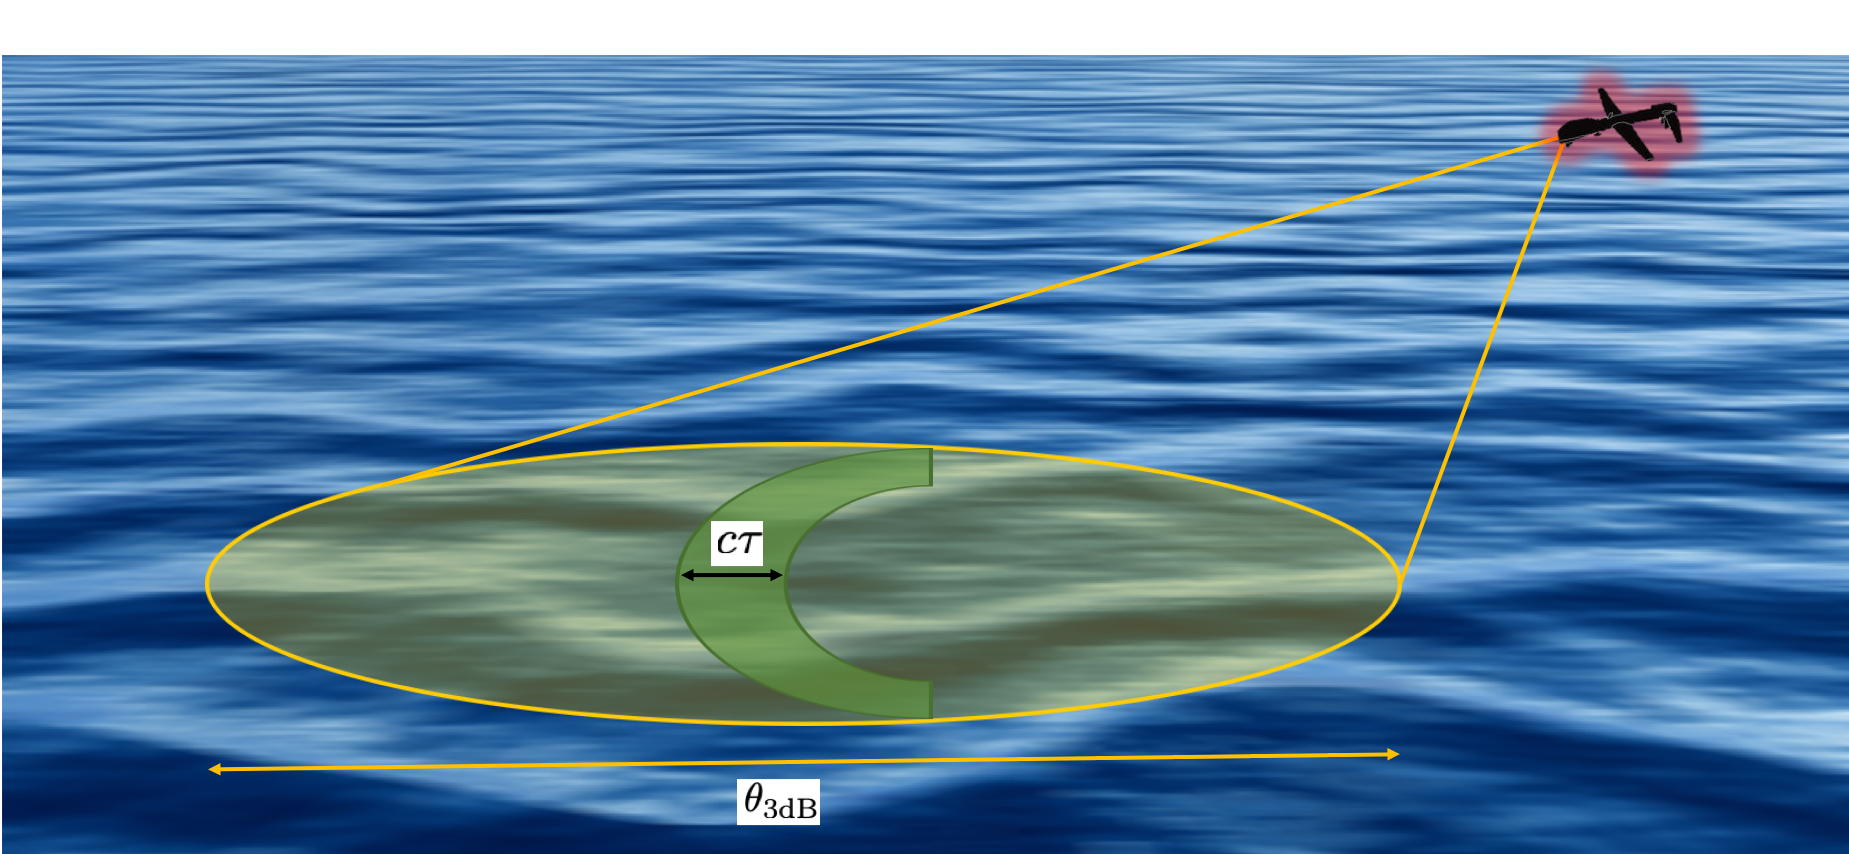
\includegraphics[width=6in]{overview.png}
\caption{Overview Diagram for Clutter Analysis.}
\label{clutter_fig1}
\end{figure}

 Fluctuations in the clutter return are driven by the changing sea surface over this projected area. Large range gate widths will average the wave motion and tend to show Rayleigh amplitude statistics. As the range gate width decreases however, individual waves become resolved and physical processes such as breaking waves start to impact the returns leading to non-Rayleigh amplitude statistics that are empirically well described by the K-distribution \cite{ward_sea_clutter}, \cite{crisp_xband}. In addition, at low grazing angles we experience wave blockage effects which also contribute to non-Rayleigh behavior.

The K-distribution was originally derived by treating the clutter return as a sum of a large number of scatterers and modeling it as a random walk in the complex plane \cite{jakeman_model_non_rayleigh}. In this work, it was shown that if the number of scatterers is allowed to fluctuate following a negative binomial distribution, then the amplitude statistics of the envelope, $E$, are governed by the K-distribution as given in Equation \ref{clutter_eq2}, with $b$ and $\nu$ as scale parameters.

\begin{gather}
\label{clutter_eq2}
P(E;b,\nu) = \frac{2b}{\Gamma(\nu)}\left(\frac{bE}{2} \right)^{\nu}K_{\nu-1}(bE)\\
b = 2\sqrt{\frac{\nu}{\left<E^2\right>}}
\end{gather}

The negative binomial distribution is required to ensure the normalized variance is finite in the limit that the number of scatterers becomes infinite, otherwise the result will reduce to the Rayleigh distribution \cite{jakeman_significance}. The K-distribution was also derived by the observation that sea clutter has 2 components: a slowly varying mean that is gamma distributed and a rapidly varying speckle component that is Rayleigh distributed in amplitude \cite{ward_sea_clutter}. These approaches derived the K-distribution in a heuristic manner and not from first principles.

As a final comment on the K-distribution, it should also be noted that in some cases (HH polarization in particular), the K-distribution is not always a good empirical fit. This has driven the development of additional compound distributions, namely the KK and KA distributions \cite{crisp_xband}.

\section{Previous Work and Plan Forward}
Previous work looked at the application of Random Matrix Theory (RMT)  to multipath fading in communications and demonstrated that the scale parameter, $\sigma$, of the Rayleigh and Rice distributions was related to the loss parameter, $\alpha$, of an open system and that the scale parameter , $\nu$, of the Rice distribution was directly driven by the dominant short orbits in the system (direct line of sight path in this case) \cite{yeh_fading} \cite{yeh_first_principles}. This work used first principles to show that wave chaos was applicable to describe fading statistics in an open system. Since clutter is also due to random scattering of electromagnetic waves, we expect to be able to show the same kind of link.

For a monostatic radar system, the transmitter and receiver are the same and we can treat this as a single channel scattering system. In addition, radar systems possess time reversal symmetry and drive us to use the Gaussian Orthogonal Ensemble (GOE) from RMT. Therefore, our starting point will be expressions developed for the statistics of the reflection coefficient, $r$, in \cite{fyodorov_statistics}. The $S$-matrix is parameterized as $S=\sqrt{r}e^{j\theta}$ in \cite{fyodorov_statistics}, but we are interested in the statistics of $|S|$ and will need to implement a change of variables to the final result.

One of the primary contributions of \cite{fyodorov_statistics} is the interpolation formula for the open system in terms of the absorption parameter, $\gamma$, and an intermediate variable, $x$, where $r = (x-1)/(x+1)$. The absorption parameter is related to the mean level spacing, $\Delta$, as $\gamma = 2\pi\Gamma/\Delta$. For the GOE case, the interpolation formula is

\begin{equation}
\label{clutter_eq3}
P_0(x) = \frac{\mathcal{N}_1}{2}\left[ A\left(\gamma\frac{x+1}{4} \right)^{1/2} +B \right]\exp\left[-\gamma\frac{x+1}{4} \right]
\end{equation}
Here, the constants are given as $A = \exp[\gamma/2]-1$, $B=1+\gamma/2 - \exp[\gamma/2]$, and $\mathcal{N}_1 = (1/2)\gamma/(A\Gamma(3/2,\gamma/2)+B\exp[-\gamma/2] )$, and $\Gamma(3/2,\gamma/2)$ is the incomplete Gamma function, $\Gamma(v,\alpha) = \int_{\alpha}^{\infty}dt \, t^{v-1}\exp[-t]$. Unfortunately, there are still significant theoretical hurdles in providing an exact expression other than in the limit of weak ($\gamma \ll 1$) or strong absorption ($\gamma \gg 1$), so Equation \ref{clutter_eq3} is still an approximation.

Equation \ref{clutter_eq3} assumes perfect coupling from the underlying chaotic system. Since this is rarely the case, we can allow the coupling constant, $T$, to be less than $1$. We can then express the distribution of the reflection coefficient in terms of a parameter $g = 2/T - 1$ \cite{fyodorov_statistics}.

\begin{equation}
\label{clutter_eq_4}
P_r(r) = \int_0^{2\pi}\frac{d\theta}{\pi(1-r)^2}P_o\left(\frac{2\left[g-\sqrt{g^2-1}\sqrt{r}\cos(\theta) \right]}{1-r} -g \right)
\end{equation}

\bibliographystyle{unsrt}     
\bibliography{clutter}
\end{document}